\subsection{Explicación del algoritmo realizado}
Los algoritmos de búsqueda local parten de una solución inicial $S_{0}$ y en cada paso intentan mejorarla. Para esto, se calculan todas las posibles variaciones de $S_{0}$ que forman una solución al problema. Al conjunto de todas estas se lo llama vecindad. 
Estos algoritmos se ejecutan siempre y cuando exista una solución, perteneciente a la vecindad, que sea mejor a la que ya teníamos. \newline \newline
Para nuestro ejercicio, utilizamos como $S_{0}$ al nodo de mayor frontera. Dicha elección se debió a que un nodo forma una clique, con lo cual es una posible solución a nuestro problema. Además, sabemos que este existe para cualquier grafo ya que la menor cantidad de nodos que se pueden ingresar en nuestro programa es uno. 
\newline Por otro lado, decidimos definir como vecindad a todas las posibles cliques que difieran en a lo sumo un nodo con nuestro $S_{0}$. Esta decisión la tomamos para que nuestra clique no quede fija alrededor del nodo inicial. Para evitarnos tener que almacenar todas las posibles cliques para posteriormente elegir la mejor, decidimos separar la vecindad en tres subconjuntos. Estos se formaron con las cliques que cumplen lo siguiente:
\begin{itemize}
\item \textbf{Tiene todos los nodos de $S_{0}$ salvo 1:} \newline En lugar de calcular todas las posibles cliques de este subconjunto, decidimos quedarnos únicamente con la clique que se obtiene de quitarle el nodo de menor grado a $S_{0}$. Esto se debe a que la frontera de una clique se puede calcular con la siguiente formula:\newline
Sea $S_{0}$ = ($V$,$E$) y n = $|$$V$$|$
\begin{equation}
  \delta(S_{0}) = \sum_{v \in V}^{} d(v) - n*(n-1)
\end{equation}
Ahora, si quitamos un nodo $v'$ de $S_{0}$, obtenemos lo siguiente:
\begin{equation}
  \delta(S'_{0}) = \sum_{v \in V/v'}^{} d(v) - (n-1)*(n-2)
\end{equation}
Como nosotros queremos encontrar el mayor \delta$(S'_{0})$, debemos quedarnos con el que tiene la sumatoria de mayor valor ya que (n-1)*(n-2) es igual para todas las cliques. Con lo cual, el nodo que debemos eliminar para poder maximizar la sumatoria, es el de menor grado.

El pseudo código de este subconjunto de la vecindad es:\newline
\begin{algorithm}[H]
    \SetAlgoLined
    \caption{quitarNodo}
    \KwIn{\textbf{Grafo} $grafo$, \textbf{Conj(Entero)} $clique$}
    \KwOut{\textbf{par(Entero,Conj(Entero))} $res$}
	
    \textbf{Entero} $minimo$ = $|$vecindad(0)$|$ \\	
    \textbf{Entero} $minimoNodo = 0$ \\
    \ForAll{$v \in$ $|clique|$}{
        $tamañoVecindad$ = $|$vecindad($v$)$|$ \\
		\If{$tamañoVecindad < minimo$}{
            $minimo$ = $tamañoVecindad$ \\
			$minimoNodo$ = $v$
	 		}}
    
    \textbf{Conj(Entero)} $cliqueQuitando$\\

    \ForAll{$v \in$ $|clique|$}{
		\If{$v \neq minimoNodo$}{
            agregar($cliqueQuitando$, $v$)
	 		}}
    
    \textbf{Entero} $fronteraRes$ = frontera($grafo$, $cliqueQuitando$)\\
    $res$ = hacerPar($fronteraRes$, $cliqueQuitando$)\\
    \textbf{devolver} $res$ \\
\end{algorithm}

Donde $frontera$ calcula la frontera del subgrafo pasado por parámetro, $agregar$ inserta un elemento en un arreglo, $vecindad$ nos devuelve todos los nodos adyacentes al nodo pasado por parámetro y $hacerPar$ genera un par con lo dos elementos pasados por parámetro. \newline


\item \textbf{Tiene todos los nodos de $S_{0}$ más uno que no pertenecía a el:} \newline
Para poder obtener la clique de frontera máxima de este subconjunto, buscamos todos los nodos del grafo que pueden formar una clique con $S_{0}$. Para esto, contamos cuantos nodos de la clique se conectan a cada nodo del grafo. Si un nodo es alcanzado por todos los que pertenecen a $S_{0}$, entonces al agregarlo, $S_{0}$ seguiría formando una clique. Una vez que tenemos a todos los posibles candidatos, calculamos la frontera de cada uno y nos quedamos con la mayor. \newline

\begin{algorithm}[H]
    \SetAlgoLined
    \caption{agregarNodo}
    \KwIn{\textbf{Grafo} $grafo$, \textbf{Conj(Entero)} $clique$}
    \KwOut{\textbf{par(Entero,Conj(Entero))} $res$}
	
    \textbf{Conj(Entero)} $bucket[$Nodos($grafo$)$]$  \\
	
    $bucket$ = marcarNodos
	
    \textbf{Conj(Entero)} $posibleClique$ = dameCandidatosAClique($bucket$)\\
   
    \textbf{Entero} $maxFrontera = 0$ \\
    \textbf{Entero} $nodo = 0$ \\

    \ForAll{$v \in$ Nodos($posibleClique$)}{
	agregar($clique$, $v$) \\
		\If{frontera($clique$) $> maxFrontera$}{
		    $maxFrontera = $ frontera($clique$)\\
		    $nodo = v$
	}
	quitar($clique$, $v$) \\}


    \eIf{ $|posibleClique| =$ 0}
	{$res$ = hacerPar(0, $clique$)}
    {	agregar($clique$, $v$) \\
	$res$ = hacerPar($maxFrontera$, $clique$) }

    \textbf{devolver} $res$ \\
\end{algorithm}

Donde $marcarNodos$ calcula para cada nodo, cuantos nodos de la clique son adyacentes a el, $dameCandidatosAClique$ nos devuelve los nodos de marcarNodos que fueron marcados por todos los nodos de la clique, $frontera$ calcula la frontera del subgrafo pasado por parámetro, $Nodos$ devuelve todos los nodos del subgrafo, $agregar$ inserta un elemento en un arreglo, $quitar$ quita un elemento en un arreglo, $vecindad$ nos devuelve todos los nodos adyacentes al nodo pasado por parámetro y $hacerPar$ genera un par con lo dos elementos pasados por parámetro. \newline

\item \textbf{Tiene todos los nodos de $S_{0}$ salvo 1 que se lo reemplaza por otro que no estaba en el:} \newline
En este subconjunto lo primero que hicimos fue quitar un nodo de $S_{0}$ y posteriormente, con la clique que nos quedo, agregarle otro. Para esto, utilizamos la función que quitaba un nodo a la clique y luego, utilizamos la función que nos calculaba el subconjunto anterior para agregar el nuevo nodo. Al hacer esto, logramos que nuestra clique no quede centrada en el nodo de mayor grado ya que este eventualmente podría dejar de formar parte de la solución.
En el caso de que la clique tenga un solo elemento, decidimos que este sea reemplazado por el nodo adyacente a el de mayor grado.  \newline
Como quitarNodo y agregarNono son dos funciones distintas, es posible que al aplicar ambas obtengamos el mismo $S_{0}$. En el caso de que esto suceda, no habría problema ya que significaría que de todas las cliques de este subconjunto, ninguna tiene mayor frontera que $S_{0}$.
\begin{algorithm}[H]
    \SetAlgoLined
    \caption{permutarNodo}
    \KwIn{\textbf{Grafo} $grafo$, \textbf{Conj(Entero)} $clique$}
    \KwOut{\textbf{par(Entero,Conj(Entero))} $res$}
	
   \textbf{Conj(Entero)} $cliqueResultante$ = segundo(quitarNodo($grafo$, $clique$)) \\

    \eIf{$|cliqueResultante| = 0$}{
	    \textbf{Entero} $nodo$ = vecinoDeMayorGrado($grafo$,$clique[0]$) \\
            agregar($cliqueRes$, $nodo$)\\
	    $res$ = hacerPar ($|$vecindad($nodo$)$|$, $cliqueRes$)	
	 		}{$res$ = agregarNodo($grafo$, $clique$)}

    \textbf{devolver} $res$ \\
\end{algorithm}
Donde $segundo$ nos devuelve el segundo elemento de una tupla,  $agregar$ inserta un elemento en un arreglo, $vecinoDeMayorGrado$ nos da el nodo de mayor grado entre todos los vecinos del vértice pasado por parámetro, $vecindad$ nos devuelve todos los nodos adyacentes al nodo pasado por parámetro y $hacerPar$ genera un par con lo dos elementos pasados por parámetro. \newline
\end{itemize}

Una vez que generamos a los tres candidatos de la vecindad, tomamos al que tiene mayor frontera y lo comparamos con $S_{0}$. Si la frontera de $S_{0}$ es menor, entonces la clique de frontera máxima de nuestra vecindad es nuestra nueva solución inicial. Caso contrario, el programa finaliza ya que ningún elemento de la vecindad puede mejorarla.

\subsection{Complejidad Temporal}
Para analizar la complejidad de nuestro algoritmo, vamos a separarlo en 5 funciones:
\begin{itemize}
\item \textbf{Generar grafo:} \newline
Para poder obtener la mayoría de las operaciones que utilizan nuestras funciones en $\mathcal{O}(1)$, generamos el grafo con los parámetros de entrada, utilizando lista y matriz de adyacencia. De esta forma, evitamos aumentar la complejidad de nuestro algoritmo. Por consiguiente, la complejidad es $\mathcal{O}(n^{2})$ ya que este es el costo de crear la matriz de adyacencia.

\item \textbf{quitarNodo:} \newline
Como podemos observar en el pseudocódigo Nº 6, lo primero que hace nuestro algoritmo es calcular mediante la función $vecindad$ ($\mathcal{O}(1)$) de la clase grafo, el tamaño de la vecindad del nodo 0. Posteriormente, hay un ciclo el cual consiste en recorrer todos los nodos de la clique($\mathcal{O}(n)$) y almacenar el de menor grado en cada paso ($\mathcal{O}(1)$).
\newline
Luego, hay un ciclo el cual nuevamente recorre todos los nodos de la clique ($\mathcal{O}(n)$) y en cada paso utiliza la función $agregar$ la cual fue implementada con $push\_back$\footnote{http://www.cplusplus.com/reference/vector/vector/push\_back/} con una complejidad de $\mathcal{O}(1)$.
\newline
Por ultimo, se calcula el valor de la frontera mediante la función $frontera$ de la clase grafo, la cual tiene una complejidad de $\mathcal{O}(n)$ y se genera un par con la solución del problema. Este par es generado mediante la función $make\_pair$\footnote{http://www.cplusplus.com/reference/utility/make\_pair/} cuya complejidad es $\mathcal{O}(1)$.
\newline
Como se puede observar, la complejidad final de $quitarNodo$ es $\mathcal{O}(n)$

\item \textbf{agregarNodo:} \newline 
Como podemos observar en el pseudocódigo Nº 7, lo primero que hace nuestro algoritmo es crear un arreglo de $n$ posiciones ($\mathcal{O}(n)$). Posteriormente, hace $marcarNodos$ el cual para cada nodo de la clique($\mathcal{O}(n)$), se fija cuales son sus vecinos mediante la función $vecindad$ ($\mathcal{O}(1)$) de la clase grafo. Luego, para cada uno de estos, ($\mathcal{O}(n)$) le suma uno a la cantidad de nodos adyacentes perteneciente a la clique que poseen. Por lo tanto, la complejidad de $marcarNodos$ es $\mathcal{O}(n^{2})$. \newline
Una vez que calcula cuantos nodos de la clique son adyacentes a cada nodo del grafo, hace $dameCandidatosAClique$. Esta función toma todos los nodos del grafo y se fija para cada uno de ellos ($\mathcal{O}(n)$) si el valor que calculo $marcarNodos$ es igual al tamaño de la clique, el cual, es calculado mediante la función size($\mathcal{O}(1)$). Por lo tanto su complejidad es ($\mathcal{O}(n)$). \newline
Posteriormente, a cada nodo de $dameCandidatosAClique$ ($\mathcal{O}(n)$), lo agrega a $S_{0}$, mediante la función $push\_back$,\footnote{http://www.cplusplus.com/reference/vector/vector/push\_back/}($\mathcal{O}(1)$). Luego, compara la frontera ($\mathcal{O}(n)$) de esta nueva clique con la frontera mas grande hasta el momento. En caso de que esta sea mayor, almacena que nodo fue el que agrego y cual es el valor de su frontera. Por ultimo, quita este nodo mediante la función $pop\_back$\footnote{http://www.cplusplus.com/reference/vector/vector/pop\_back/} cuya complejidad es $\mathcal{O}(1)$). El costo de realizar esto es $\mathcal{O}(n^{2})$. \newline
Una vez que tiene la solución, genera un par con esta mediante la función $make\_pair$\footnote{http://www.cplusplus.com/reference/utility/make\_pair/} cuya complejidad es $\mathcal{O}(1)$.
\newline
Como se puede observar, la complejidad final de $agregarNodo$ es $\mathcal{O}(n^{2})$

\item \textbf{permutarNodo:} \newline 
Como podemos observar en el pseudocódigo Nº 8, nuestro algoritmo hace dos cosas. Primero le quita un nodo a la clique mediante la función $quitarNodo$ cuya complejidad es $\mathcal{O}(n)$. Posteriormente, se fija si el resultado de $quitarNodo$ es vacío o no. \newline
En el caso de que sea vacío, calcula mediante $vecinoDeMayorGrado$ cual de todos los nodos adyacentes al pasado por parámetro tiene mayor grado. Para esto, recorre todos los nodos adyacentes y compara en $\mathcal{O}(1)$ sus grados, por lo tanto su complejidad es $\mathcal{O}(n)$. Una vez que tiene la solución, la coloca en un arreglo mediante $push\_back$ y genera un par con esta mediante la función $make\_pair$ cuya complejidad es $\mathcal{O}(1)$.
\newline
Si por el contrario, la clique no estaba vacía, obtiene la solución mediante la función $agregarNodo$ cuya complejidad es $\mathcal{O}(n^{2})$
\newline
Como se puede observar, la complejidad final de $permutarNodo$ es $\mathcal{O}(n^{2})$

\item \textbf{busquedaLocal:} \newline 

\begin{algorithm}[H]
    \SetAlgoLined
    \caption{busquedaLocal}
    \KwIn{\textbf{Grafo} $grafo$, \textbf{Entero} $m$}
    \KwOut{\textbf{Conj(Entero)} $res$}
	
    agregar($res$, nodoDeMayorGrado($grafo$))\\
    	
    \For{i = 0  \textbf{to} i $<$ m}{
        \textbf{par(Entero, Conj(Entero))} $solucionParcial = $ agregarNodo($grafo, res$)\\
	\If{primero($solucionParcial$)$ < $primero(quitarNodo($grafo$, $res$))}{
            $solucionParcial = $ quitarNodo($grafo$, $res$)\\
	 		}
    	\If{primero($aux$)$ < $primero(permutarNodo($grafo$, $res$))}{
            $solucionParcial = $ permutarNodo($grafo$, $res$)\\
	 		}
	\eIf{primero($solucionParcial$)$ > $frontera($res$)}{
            $res = $ primero($solucionParcial$)\\
	 		}{$salir del ciclo$}
	}
    \textbf{devolver} $res$ \\
\end{algorithm}

Como se observa en el pseudocódigo Nº 9, nuestro algoritmo coloca en $res$ el nodo de mayor grado del grafo. Esta función tiene complejidad $\mathcal{O}(n)$. Posteriormente, ejecuta agregarNodo ($\mathcal{O}(n^{2})$), quitarNodo ($\mathcal{O}(n)$) y permutarNodo ($\mathcal{O}(n^{2})$). Estas tres funciones se ejecutan como máximo $m$ veces. Esto se debe a que la frontera debe ser siempre creciente en la cantidad de aristas. Por lo tanto, en cada paso a lo sumo puede crecer en una unidad llegando a un máximo de $m$. Con lo cual, la complejidad del ciclo es $\mathcal{O}(n^{2})$ * $\mathcal{O}(n^{2})$
\newline
Como se puede observar, la complejidad final de $busquedaLocal$ es $\mathcal{O}(n^{4})$

\subsection{Instancias problemáticas}
Si observamos nuestro algoritmo, podemos notar que este siempre arranca por el nodo de mayor grado. Posteriormente, se va moviendo, en cada iteración, a una clique la cual dista a lo sumo en una unidad con la clique actual. Teniendo en cuenta esto, nuestro algoritmo va a encontrar la solución exacta siempre y cuando haya cliques, las cuales generen fronteras cada vez mas grande, entre el nodo de mayor grado y la clique de frontera máxima.
\newline
Veamos que sucede en el caso en el que la solución no es la óptima. Como ya dijimos antes, partimos del nodo de grado máximo, por lo tanto d($S_{0}$) $\leq$ frontera($S$). Por otro lado, se que los grados de los nodos que conforman $S$ no pueden ser mayores a d($S_{0}$). Esto se debe a que si lo fueran, estos serian el $S_{0}$ de nuestro algoritmo. Como quiero ver que tan mala es la solución que obtuve, voy a buscar la solución con máxima frontera. Para esto, calculemos cuanto vale la frontera de una clique genérica. \newline
En primer lugar, notemos que para maximizar la frontera, debemos tener todos los nodos de la clique con la mayor cantidad de aristas posibles. Como vimos anteriormente, el grado de los nodos no puede superar a d($S_{0}$). Luego, para una clique de $c$ nodos de grado d($S_{0}$), obtenemos que su frontera es:
\begin{equation}
  frontera(S) = d(S_{0}) * c - (c - 1) * c
\end{equation} 
Esta es la frontera mas grande que se puede encontrar para cada valor de $c$.
\newline 
Ahora, veamos cuanto es el máximo error que se puede cometer al no encontrar la solución óptima. Para esto, debemos restarle a la formula anterior d($S_{0}$). Esto se debe a que es la menor frontera que encuentra nuestro algoritmo.
\begin{equation}
  máximo\ error = d(S_{0}) * c - (c - 1) * c - d(S_{0}) 
\end{equation} 
Saco factor común d($S_{0}$)
\begin{equation}
  máximo\ error = d(S_{0}) * (c - 1) - (c - 1) * c 
\end{equation} 
Saco factor común (c - 1)
\begin{equation}
  máximo\ error = (c - 1) * (d(S_{0}) - c) 
\end{equation} 
Calculemos cual es el valor de c que maximiza esta función. Derivemos con respecto a $c$
\begin{equation}
  máximo\ error' = (d(S_{0}) - c) - (c - 1)
\end{equation} 
igualemos a 0 y despejemos
\begin{equation}
  c = \frac{1 + d(S_{0})}{2}
\end{equation} 
Si derivo una vez mas y evalúo en c = $\frac{1 + d(S_{0})}{2}$, obtengo que:
\begin{equation}
  máximo\ error'' = -2 < 0
\end{equation}
Por lo tanto es máximo.\newline \newline
Veamos cual es el máximo error que se puede obtener.

\begin{equation}
  máximo\ error = d(S_{0}) * \frac{1 + d(S_{0})}{2} - (\frac{1 + d(S_{0})}{2} - 1) * \frac{1 + d(S_{0})}{2} - d(S_{0}) 
\end{equation} 
\begin{equation}
  máximo\ error = \frac{1 - 2 * d(S_{0}) + d(S_{0})^{2}}{4} 
\end{equation}

veamos 2 casos en donde nuestro algoritmo no encuentra la solución óptima:
\begin {itemize}
\item
\textbf{Formato de entrada:}

$$14\ \  14$$
$$1\ \  2$$
$$1\ \  3$$
$$1\ \  4$$
$$1\ \  5$$
$$1\ \  6$$
$$6\ \  7$$
$$7 \ \ 8$$
$$8\ \  9$$
$$9\ \  7$$
$$8\ \  10$$
$$8\ \  11$$
$$9\ \  12$$
$$9\ \  13$$
$$7\ \  14$$


\textbf{Formato de salida:}
$$5\ \   1\ \   1$$
\begin{figure}[H] %[h] Aqui [b] para button [t] para top
\begin{center}
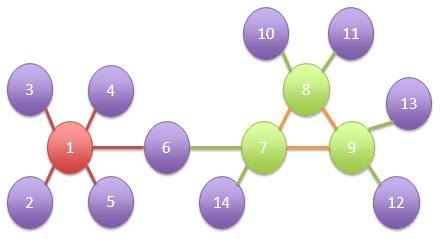
\includegraphics[width=250pt]{../imgs/ej1local.jpg}
\caption{Ejemplo}
\end{center}
\end{figure}
Como se puede notar en el grafico, la frontera máxima según nuestro algoritmo es 5 (aristas rojas) cuando la exacta es en realidad 6 (aristas verdes) y esta conformada por los nodos 7 8 9 . esto se debe a que el nodo de mayor grado es el 1 y dista en dos nodo de la clique máxima. 
\newline
comprobemos que esto satisface nuestra cota:
\begin{equation}
  máximo\ error = \frac{1 - 2 * 5) + 5^{2}}{4} = 4
\end{equation}
\begin{equation}
  algoritmo\ exacto - heurística = 6 - 5 = 1
\end{equation}

\item
\textbf{Formato de entrada:}

$$17\ \  17$$
$$1\ \  2$$
$$1\ \  3$$
$$1\ \  4$$
$$1\ \  5$$
$$1\ \  6$$
$$6\ \  7$$
$$7 \ \ 8$$
$$8\ \  9$$
$$9\ \  7$$
$$8\ \  10$$
$$8\ \  11$$
$$9\ \  12$$
$$9\ \  13$$
$$7\ \  14$$
$$7\ \  15$$
$$8\ \  16$$
$$9\ \  17$$

\textbf{Formato de salida:}
$$5\ \   1\ \   1$$
\begin{figure}[H] %[h] Aqui [b] para button [t] para top
\begin{center}
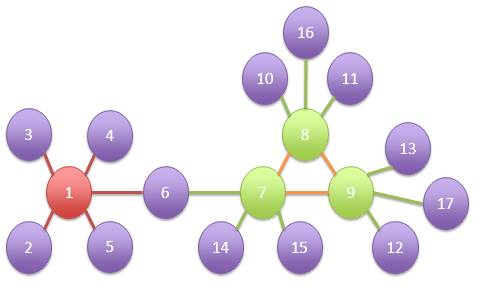
\includegraphics[width=250pt]{../imgs/ej2local.jpg}
\caption{Ejemplo}
\end{center}
\end{figure}
Como se puede notar en el gráfico, la frontera máxima según nuestro algoritmo es 5 (aristas rojas) cuando la exacta es en realidad 9 (aristas verdes) y esta conformada por los nodos 7 8 9 . esto se debe a que el nodo de mayor grado es el 1 y dista en dos nodo de la clique máxima.
\newline
comprobemos que esto satisface nuestra cota:
\begin{equation}
  máximo\ error = \frac{1 - 2 * 5 + 5^{2}}{4} = 4
\end{equation}

\begin{equation}
  algoritmo\ exacto - heurística = 9 - 5 = 4
\end{equation}
\end{itemize}

\subsection{Experimentación}

